%% ------------------------------------------------------------------- %%
%% ------------------------------------------------------------------- %%
%% ------------------------------------------------------------------- %%
%% ------------------------------------------------------------------- %%
\chapter{Propuesta}
\label{cap:propuesta}

\lhead{\emph{Propuesta}} 
%% ------------------------------------------------------------------- %%
%% ------------------------------------------------------------------- %%
%% ------------------------------------------------------------------- %%
%% ------------------------------------------------------------------- %%
%% ------------------------------------------------------------------- %%
%% ------------------------------------------------------------------- %%

%% -------------------------------------------------------------------- %%
%% -------------------------------------------------------------------- %%


La detección de neoantígenos es un proceso largo, descrito anteriormente. Debido a esto, esta investigación se ha centrado en la predicción de la unión pMHC, porque es una de las etapas con mayor investigación en el estado del arte y sin embargo, los resultados aún carecen de buen desempeño. En resumen, en este trabajo hemos realizado \textit{fine-tuning} a modelos \textit{BERT}, para la tarea de predicción de la unión pMHC. En este capítulo, se explica el proceso de \textit{fine-tuning} utilizado, los modelos pre-entrenados TAPE, ESM2 y ProtBert. Además, se aplico una metodología de congelamiento de capas y \textit{Gradient Accumulation Steps}. 




\begin{comment}
	

\section{Predicción de la afinidad peptido-MHC (peptide-MHC binding)}

La propuesta se inspira en los trabajos de \cite{cheng2021bertmhc} y \cite{hashemi2022improved}. Ambos proponen el uso de \textit{transfer  learning} a partir de los modelos pre-entrenados BERT \citep{devlin2018bert} y ESM-1b \citep{rives2021biological} respectivamente. \\


El modelo \textit{Bidirectional Encoder Representations from Transformers.} (BERT), fue diseñado para el pre-entrenamiento de representaciones bidireccionales de textos no etiquetados. Este modelo fue diseñado inicialmente para el procesamiento natural del lenguaje, pero en el trabajo de \cite{rao2019evaluating}, se planteó su uso para secuencias de aminoácidos. Es así que \cite{rao2019evaluating} entrenan BERT con 31 millones de secuencias de proteínas y llaman a su propuesta \textit{Tasks Assessing Protein Embeddings} (TAPE).\\

Recientemente, Facebook desarrolla el modelo ESM-1b \citep{rives2021biological}. La propuesta se basa en el modelo RoBERTa \citep{liu2019roberta}, la cuál es una optimización de BERT. Luego, ESM-1b fue entrenado con la base de datos Uniref50 \citep{suzek2015uniref}, esta base de datos cuenta con aproximadamente 250 millones de secuencias de proteínas. En este caso, se realizó un entrenamiento no supervisado, se ocultaron las etiquetas referentes a la estructura o función de las proteínas.\\

Entonces, la propuesta de la tesis se basa en utilizar \textit{transfer learning} del modelo pre-entrenado ESM-1b, luego se va a utilizar otra red neuronal paralela que se alimente de datos físico-químicos de los aminoácidos. Se propone utilizar las propiedades físico-químicas de los aminoácidos, porque en varios ensayos clínicos se ha comprobado que influyen en la predicción \textit{peptide-MHC binding} y \textit{pMHC-TCR presentation} \citep{gopanenko2020main, borden2022cancer}. Luego, las dos redes neuronales paralelas se unirán en una red neuronal totalmente conectada (ver Figura \ref{fig:proposal}). El objetivo, es aprovechar las propiedades físico-químicas de los aminoácidos para mejorar la afinidad \textit{peptide-MHC}.

Para los entrenamientos y experimentos se utilizará la base de datos HLA3D \citep{li2022hla3d}, esta contiene información de 1296 aminoácidos. Luego, también utilizaremos las muestras recolectadas de \cite{hashemi2022improved}.
\end{comment}

\section{Metodología}

Esta investigación se  enfoca en la tarea de predecir la unión pMHC, descrito en la etapa 3.1 del proceso general para generar vacunas personalizadas basadas en neoantígenos (ver Figura \ref{fig:proposal}). Se ha evaluado  seis modelos \textit{Transformer}s pre-entrenados en diversas tareas de Proteómica como: predicción de estructura de proteínas, predicción de la función de proteínas, etc. Los modelos BERT son: TAPE \citep{rao2019evaluating}, ProtBert-BFD \citep{elnaggar2021prottrans} y ESM2 \citep{lin2023evolutionary} ( compuesto por ESM2(t6), ESM2(t12), ESM2(t30), ESM2(t33)). Durante la evaluación se realizó \textit{fine-tuning} a los modelos agregando un bloque de BiLSTM al final, de igual forma que lo realizó HLAB \citep{zhang2022hlab}, describiremos a detalle ste proceso mas adelante. También se evaluó el uso de \textit{Gradient Accumulation Steps} (GAS) y el uso de una metodología para congelar las capas del modelo BERT con el objetivo de reducir el tiempo de entrenamiento, consumo de memoria y disminuir el problema de \textit{vanish gradient}. 






\begin{figure}[H]
	\centering
	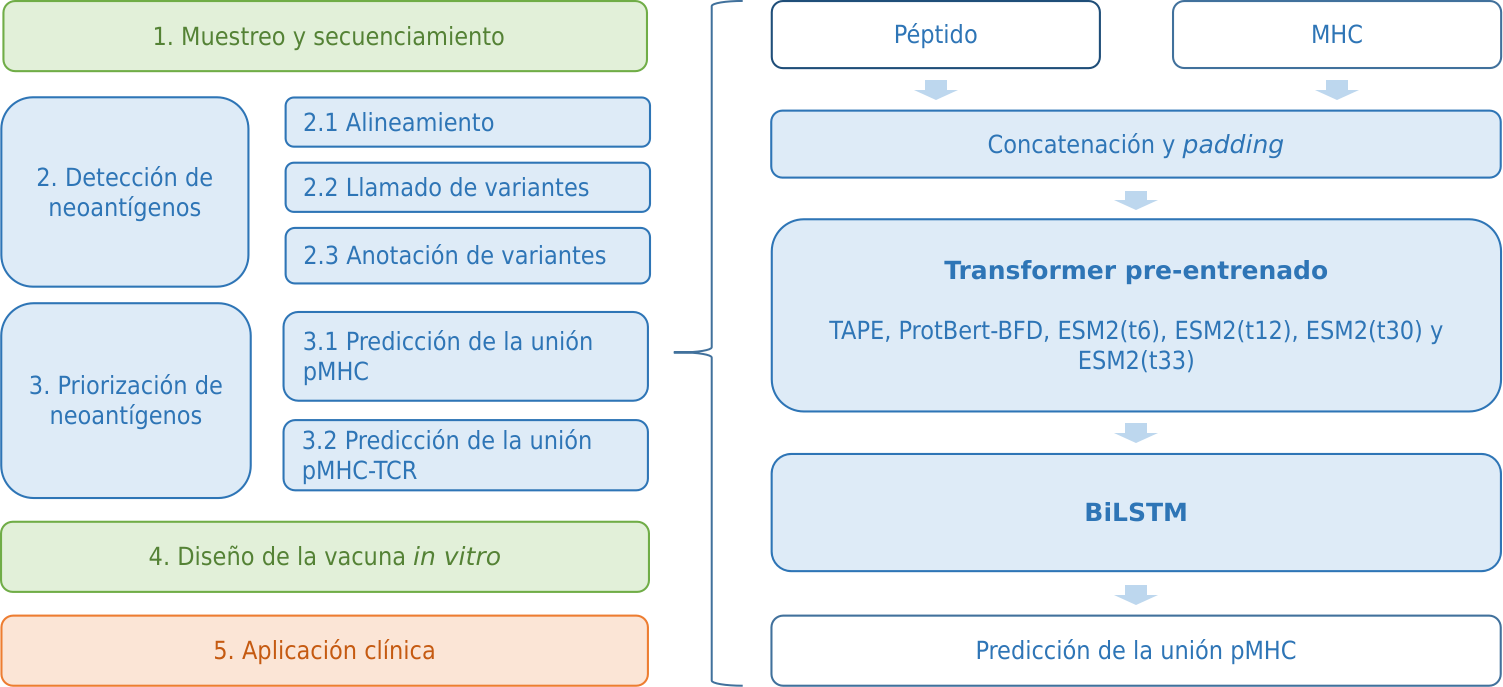
\includegraphics[width=\textwidth]{../img/proposal/proposal}	
	\caption{Propuesta de \textit{transfer learning} de ESM-1b y una red neuronal paralela para la predicción de la afinidad entre un péptido y MHC (peptide MHC binding).}
	\label{fig:proposal}
\end{figure}

En la Figura \ref{fig:proposal}, describimos la propuesta para la predicción del enlave pMHC para MHC de clase I. Primero tomamos como entrada el péptido y el MHC-I. Estas son secuencias de proteínas, el peptido tiene una longitud entre 8 a14 aminoácidos; mientras que para el MHC se ha utilizado pseudosecuencias con una longitud de 34 aminoácidos. Luego, estós aminoácidos son codificados utilizando one-hot encoding (ver Figure \ref{fig:onehot}). Luego estos aminoácidos son concatenados y son recibidos por el modelo BERT (modelo pre-entrenado). Finalmente, luego del bloque BERT prosigue un bloque de capas BiLSTM y finalmente una capa lineal para clasificar o predecir la unión entre el péptido y el MHC.

\begin{figure}[H]
	\centering
	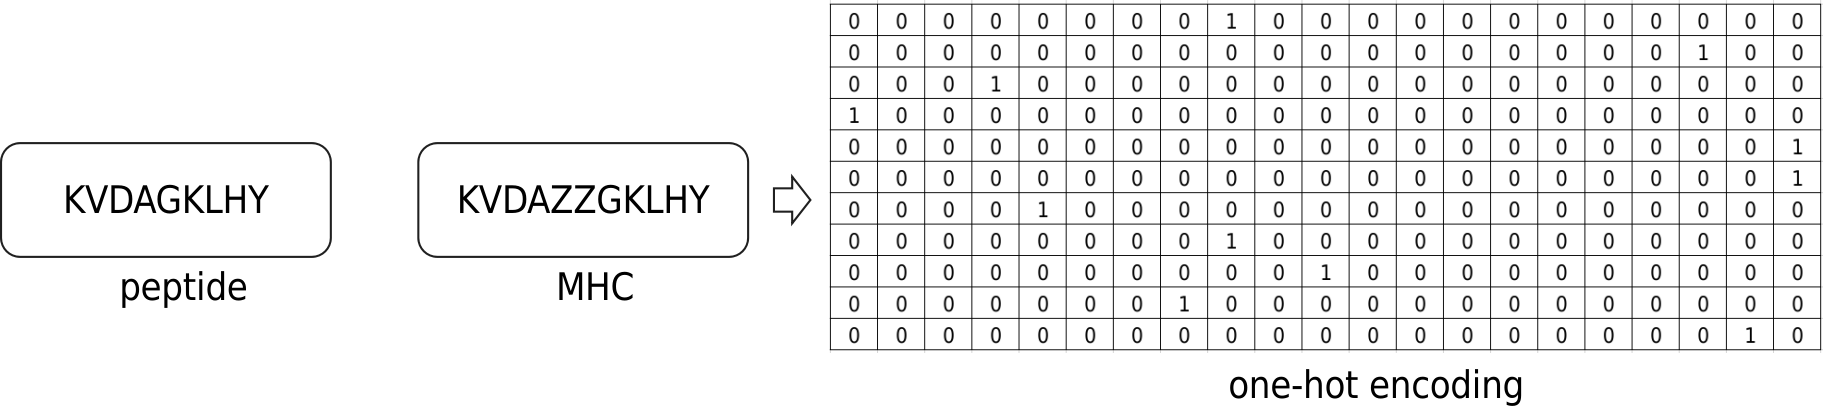
\includegraphics[width=\textwidth]{../img/proposal/onehot}	
	\caption[Ejemplo de codificación de aminoácidos con \textit{one-hot encoding}]{Ejemplo de codificación de aminoácidos con \textit{one-hot encoding}. Cada aminoácido es representado con un vector de ceros u un 1, según el tipo de aminoácido de veinte posibles aminoácidos.}
	\label{fig:onehot}
\end{figure}

\section{Modelos BERT}

El modelo \textit{Bidirectional Encoder Representations from Transformers} (BERT) fue presentado en el artículo ``BERT: Pre-training of Deep Bidirectional Transformers for Language Understanding'' \cite{devlin2018bert}. Este modelo se trata de un Transformer bidireccional preentrenado con información de las bases de datos de Libros de Toronto y Wikipedia. El modelo está compuesto por un \textit{encoder} y un \textit{decoder} (ver Figura \ref{fig:bert_paper}), donde el \textit{encoder} tiene la funcionalidad de codificar los \textit{tokens}, mientras que el \textit{decoder} los decodifica y los convierte nuevamente a texto. Adicionalmente, los modelos de lenguaje tradicionales procesan el texto de manera secuencial, ya sea de izquierda a derecha o de derecha a izquierda. Este método limita la capacidad del modelo para comprender el contexto inmediato que precede a la palabra objetivo. BERT utiliza un enfoque bidireccional que considera tanto el contexto izquierdo como el derecho de las palabras en una oración. En lugar de analizar el texto secuencialmente, BERT examina todas las palabras en una oración simultáneamente.

\begin{figure}[H]
	\centering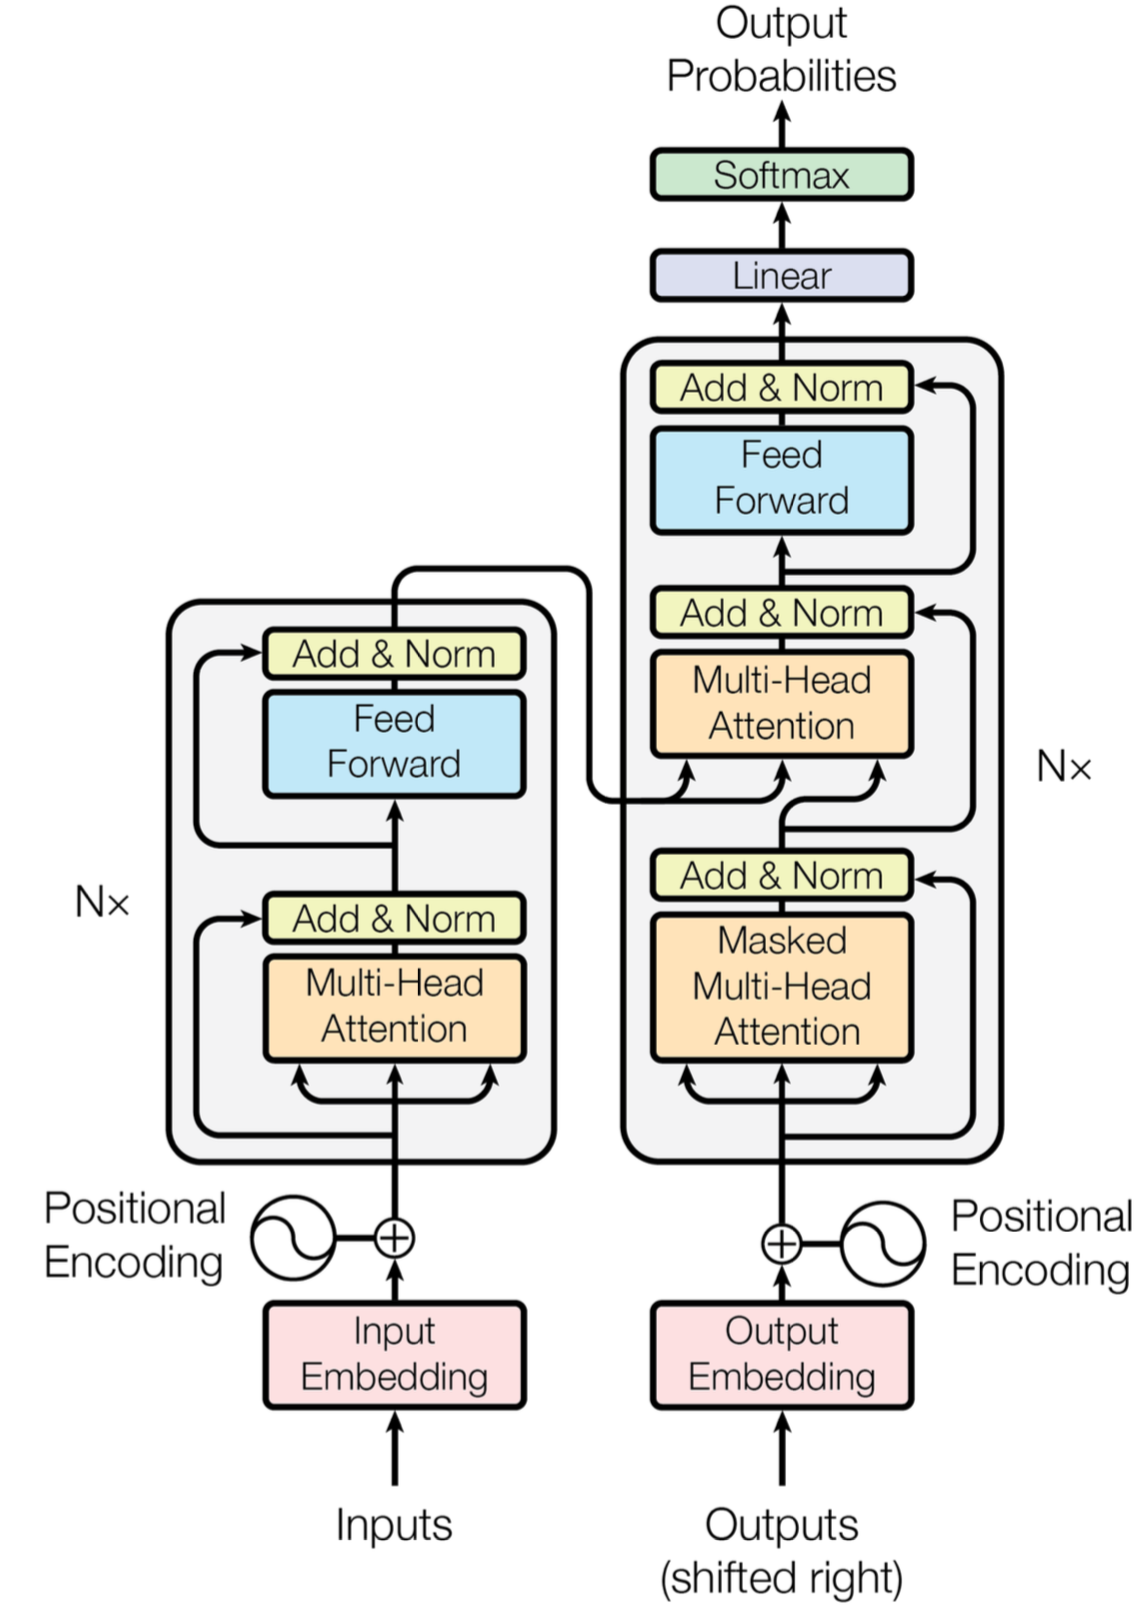
\includegraphics[width=0.7\textwidth]{../img/proposal/bert}
	\caption[Aquitectura del modelo BERT]{Arquitectura del modelo BERT diferenciado los \textit{encoders} y \textit{decoders}. Fuente: \cite{devlin2018bert}.}
	\label{fig:bert_paper}
\end{figure}


BERT está impulsado por una potente arquitectura de red neuronal conocida como \textit{Transformers}. Esta arquitectura incorpora un mecanismo llamado \textit{self-attention}, lo que permite a BERT ponderar la importancia de cada palabra en función de su contexto, tanto precedente como sucesivo. Esta conciencia contextual dota a BERT con la capacidad de generar incrustaciones de palabras contextualizadas, que son representaciones de palabras considerando sus significados dentro de las oraciones. 

\subsection{Modelos de lenguaje de preoteínas}

El modelo BERT ha permitido grandes avances en el área de procesamiento natural del lenguaje y también se ha extendido hacia otras aplicaciones, como el análisis de secuencias de aminoácidos (proteínas). Por ejemplo, en la Figura \ref{fig:aminoacids}, mostramos un ejemplo de una cadena de aminoácidos y cómo se forma a partir de la secuencia mRNA. Cada tres bases conforman un posible aminoácido y tenemos veintidós en total.


\begin{figure}[H]
	\centering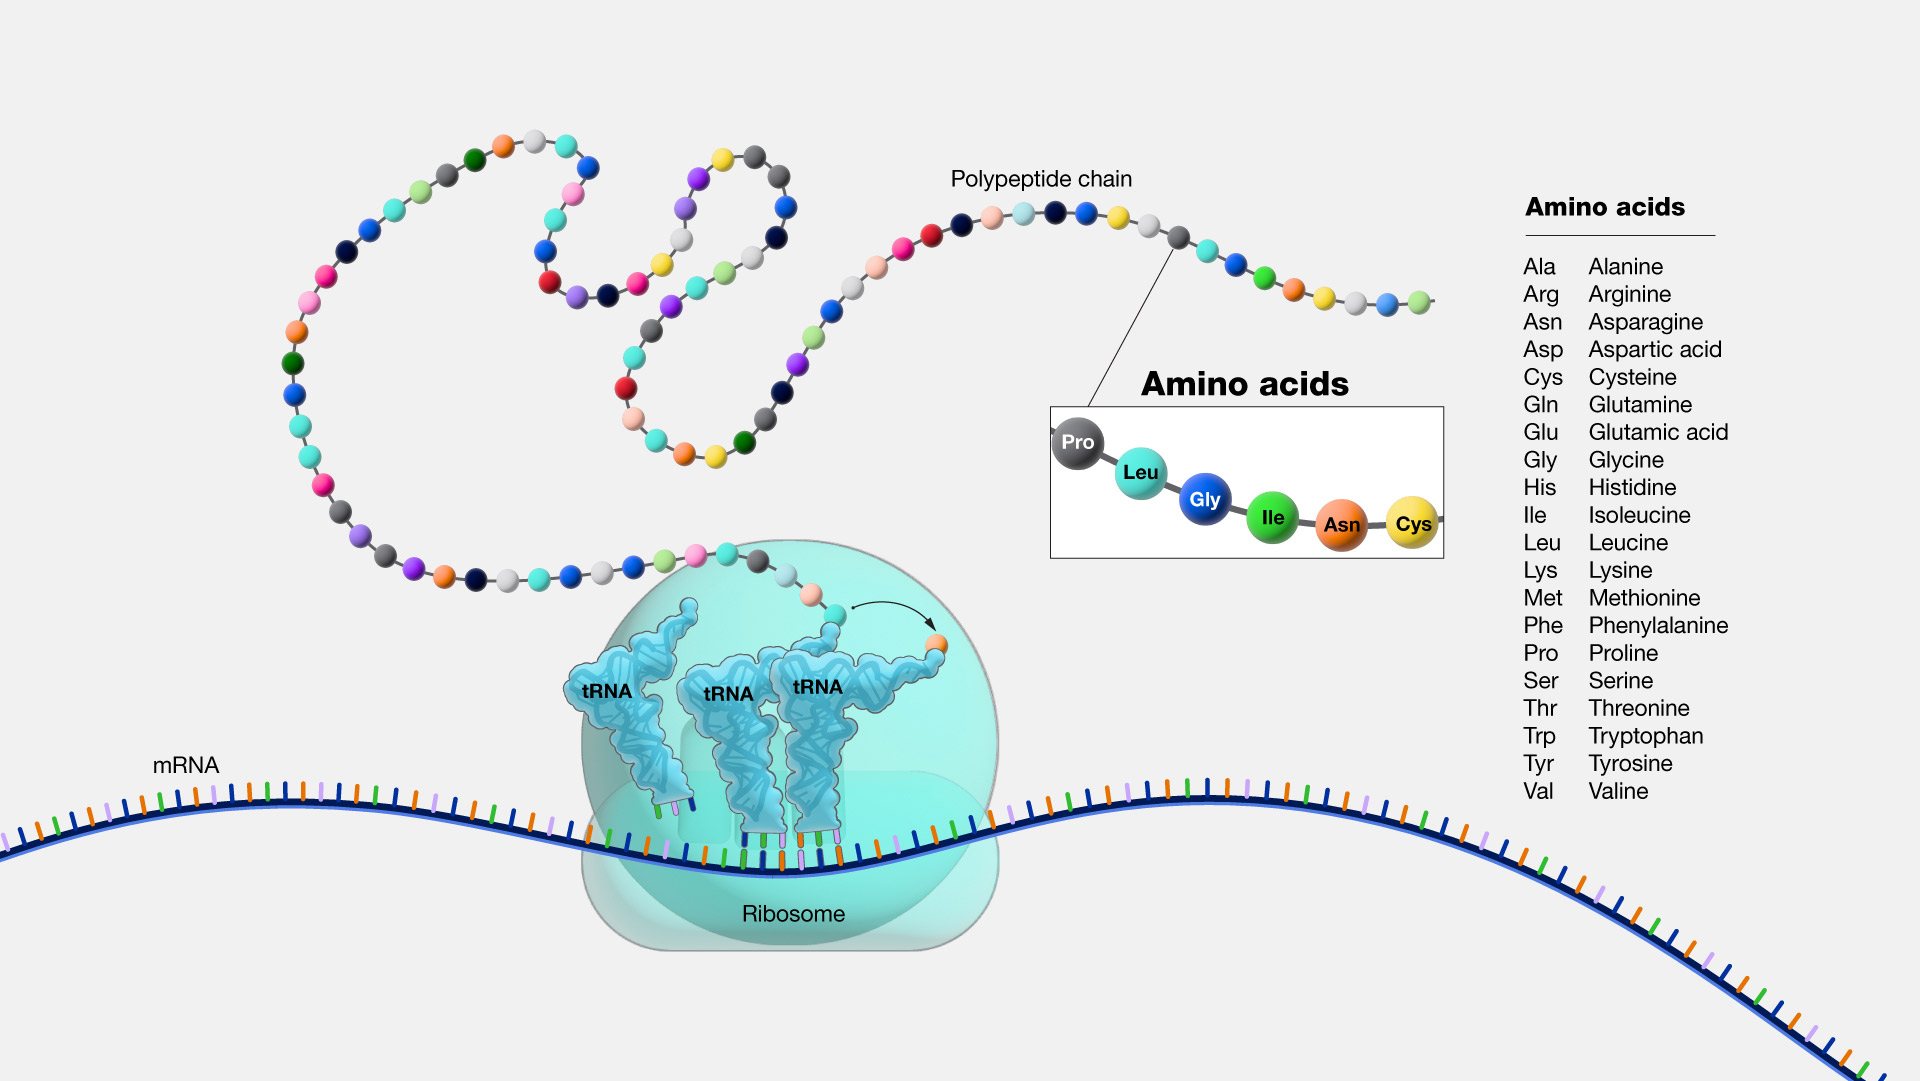
\includegraphics[width=\textwidth]{../img/proposal/amino-acids}
	\caption[Ejemplo de traducción de aminoácidos]{Ejemplo de como ocurre la traducción de aminoácidos a partir de una secuencia mRNA. Cada tres bases conforman un aminoácido y en total tenemos veintidos diferentes aminoácidos. Fuente: \cite{nih_aminoacids_2024}.}
	\label{fig:aminoacids}
\end{figure}



\begin{figure}[H]
	\centering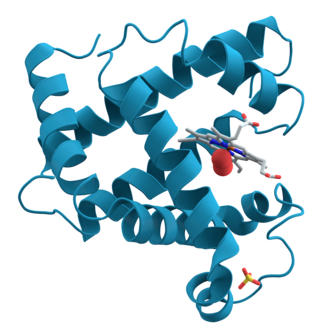
\includegraphics[width=0.45\textwidth]{../img/proposal/myoglobin}
	\caption[Estructura 3D de la proteína Mioglobulina]{Estructura 3D de la proteína Mioglobulina. Esta estructura 3D esta compuesta por 154 aminoácidos: \textit{MGLSDGEWQ LVLNVWGKVE ADIPGHGQEV LIRLFKGHPE TLEKFDKFKH LKSEDEMKAS EDLKKHGATV LTALGGILKK KGHHEAEIKP LAQSHATKHK IPVKYLEFIS ECIIQVLQSK HPGDFGADAQ GAMNKALELF RKDMASNYKE LGFQG}. Fuente: \cite{uniprotkb}, identificación P02144.}
	\label{fig:myoglobin}
\end{figure}

Según la cadena de aminoácidos, la estructura y función de una proteína es determinada \citep{rastogi2022bioinformatics,kihara2017protein,rangwala2010introduction}. Por ejemplo la secuencia de aminoácidos: \textit{MGLS DGEWQ LVLNV WGKVE ADIPG HGQEV LIRL FKGHPE TLEKF DKFKH LKSE DEMKAS EDLK KHGATV LTALG GILKK KGHH EAEIKP LAQSH ATKHK IPVKY LEFIS ECIIQ VLQSK HPGD FGADAQ GAMNK ALELF RKDM ASNYKE LGFQG}, representa la proteína Mioglobulina (ver Figura \ref{fig:myoglobin}). Según la posición de cada aminoácido y el tamaño de la secuencia, la proteína cumple con cierta función. Entonces, si una mutación ocurre a nivel de aminoacidos por ende la función de la proteína se vera afectada, este es origen de varios tipos de cancer \citep{xie2023neoantigens,biswas2023designing}. Por ejemplo, en la Figura \ref{fig:mutabind}, presentamos  una mutación por sustitución, donde el aminoácido K cambio por E, este cambio pequeño modifico la estructura y función de la proteína.

\begin{figure}[H]
	\centering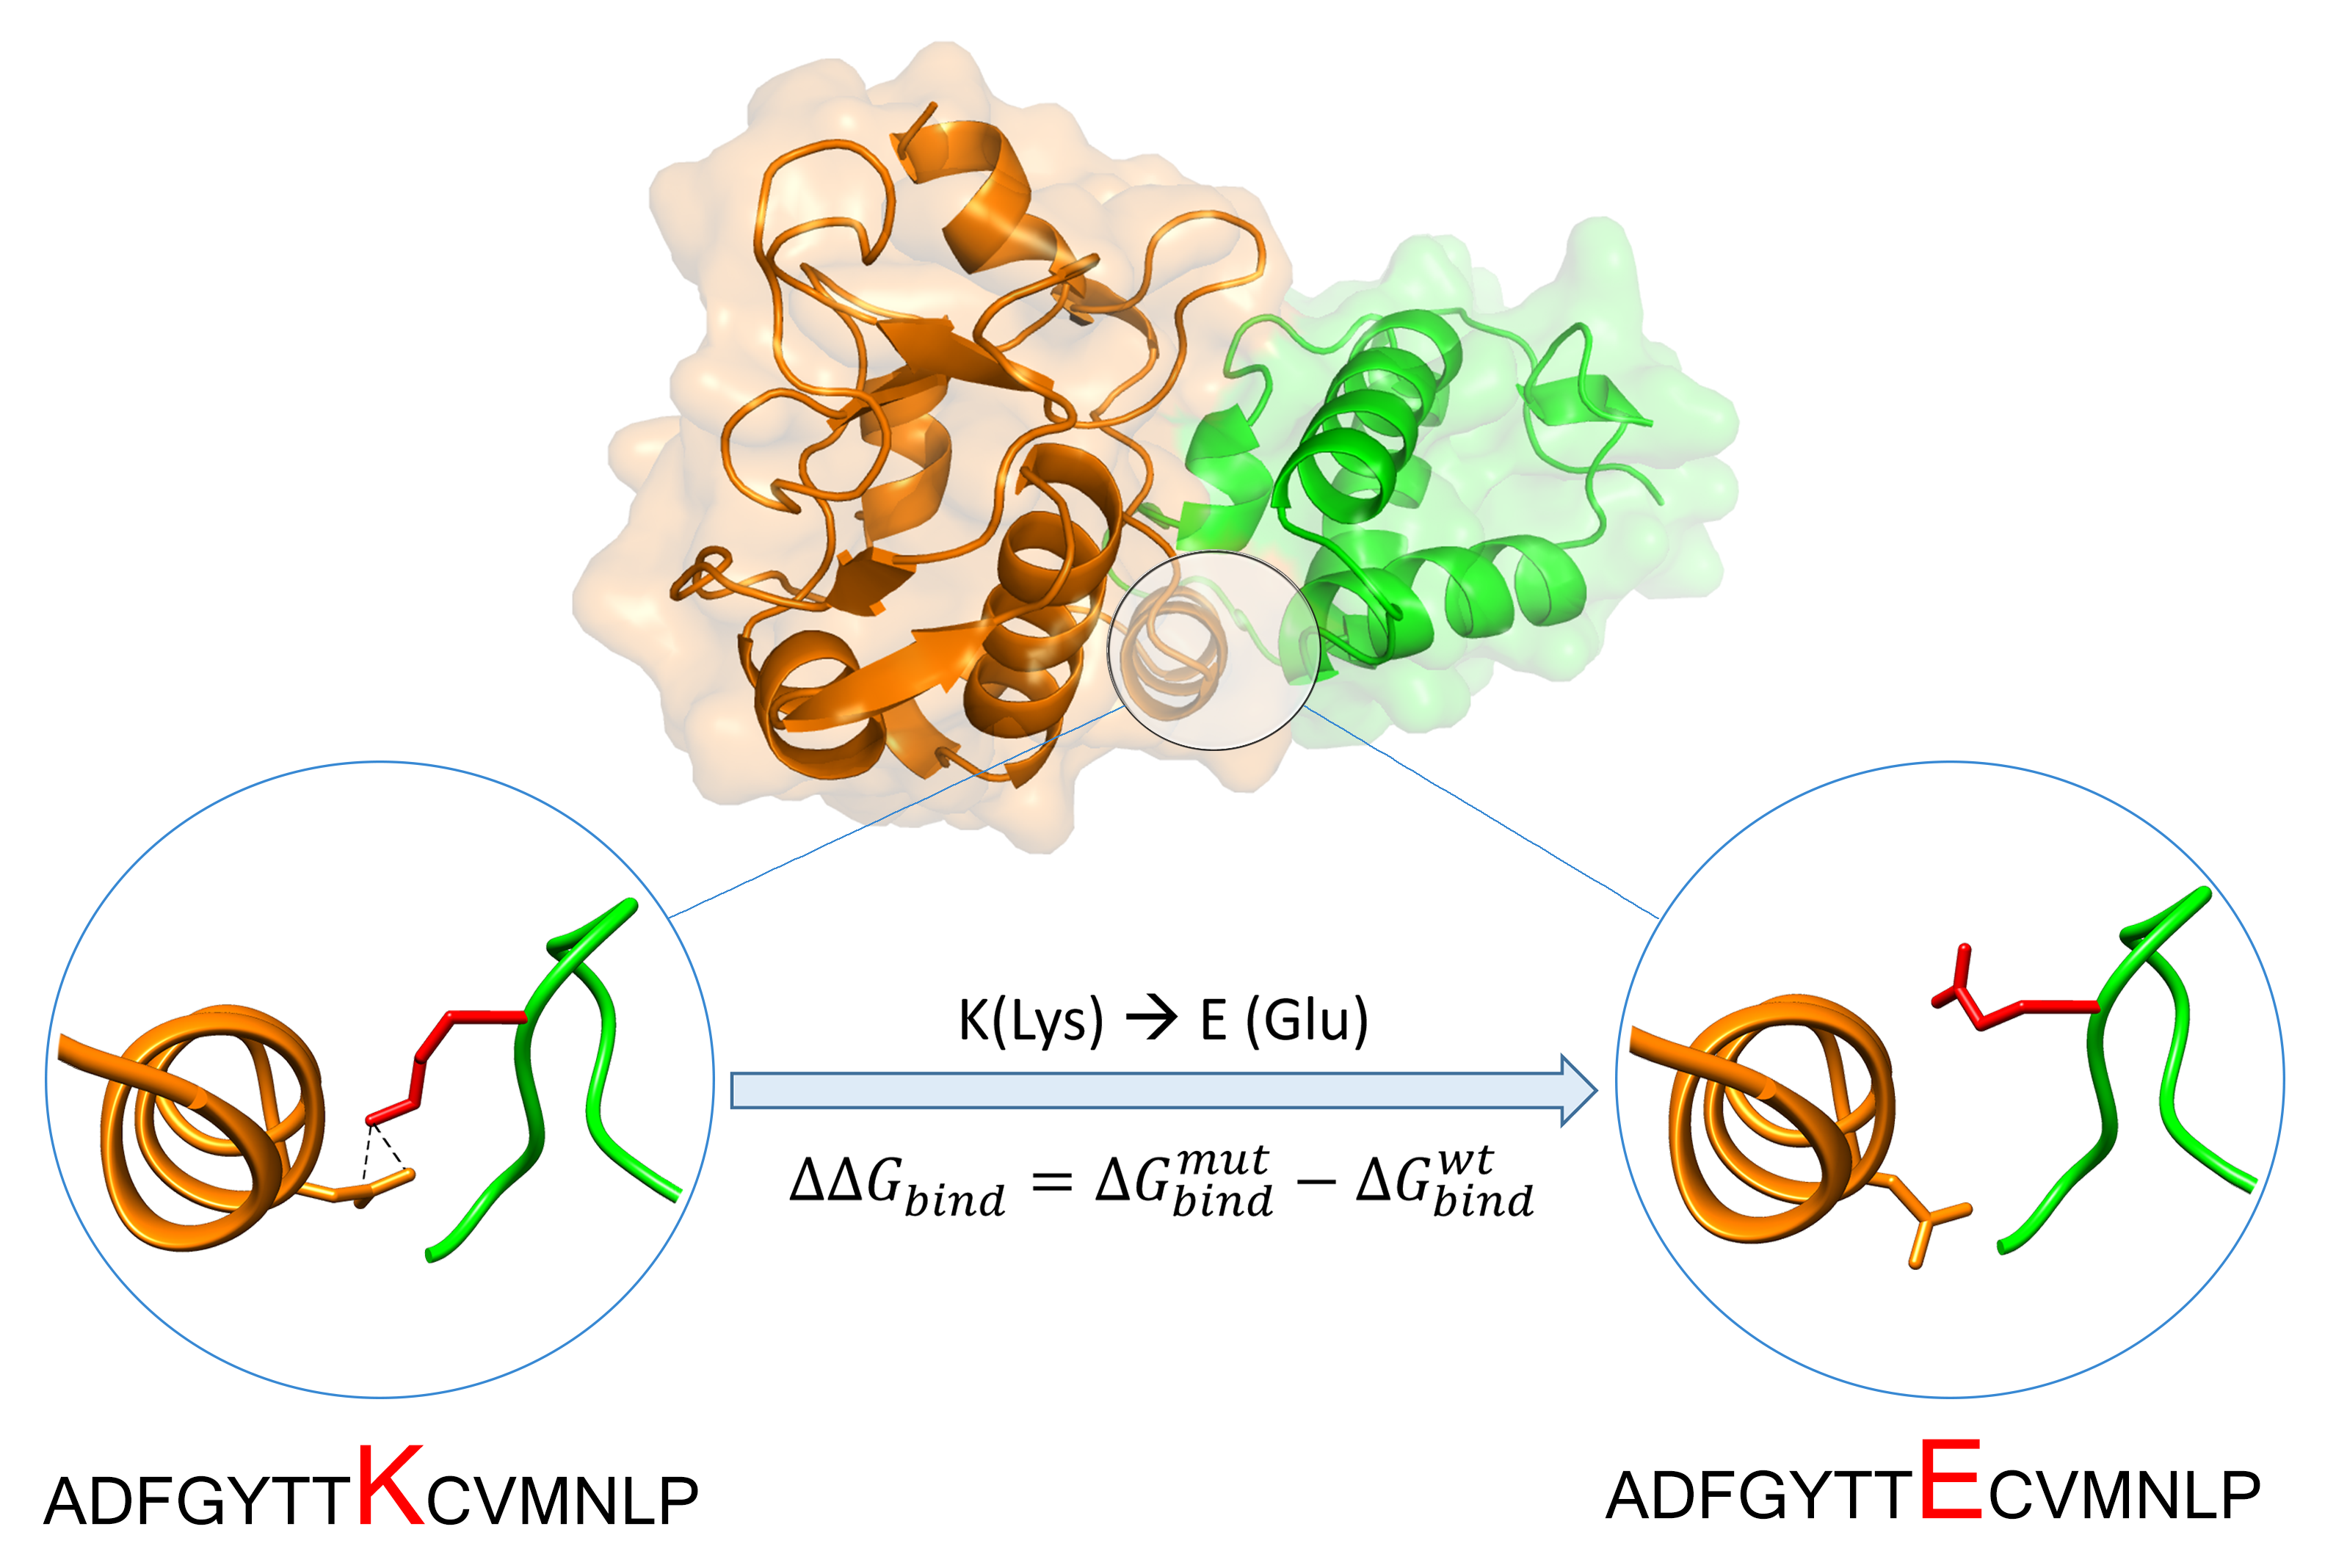
\includegraphics[width=0.7\textwidth]{../img/proposal/mutabind}
	\caption[Estructura 3D de una proteína normal y una proteína mutada]{Estructura 3D de una proteína normal y una proteína mutada. La mutación ocurrio en el aminoácido K, que cambio y se volvio el aminoácido E. Esta mutación genero un cambio en la estructura y función de la proteína. Fuente: \cite{mutabind2024}}
	\label{fig:mutabind}
\end{figure}

Entonces, una secuencia de aminoácidos es muy similar a una cadena de texto. En una cadena de texto, las palabras pueden ser los \textit{tokens}; mientras que en la secuencia de aminoácidos, cada aminoácido sería un \textit{token}. Además, el orden de los aminoácidos determina la estructura y función de las proteínas. Basándonos en estas premisas, varios autores han considerado el estudio de proteínas de manera similar a una tarea de procesamiento natural del lenguaje. De esta forma, existen trabajos que han utilizado Transformers para diversas tareas en Proteómica, como la predicción de la estructura de una proteína, la predicción de la función y del \textit{contact map}, así como la predicción del enlace entre dos proteínas. Esta área de estudio es tan importante que, de manera similar a los modelos de lenguaje grandes como Llama2 y Mistral, se han entrenado modelos BERT con millones de secuencias de proteínas. Incluso, se han utilizado metodologías similares para el entrenamiento de modelos de lenguaje. Por ejemplo, tradicionalmente los modelos de lenguaje utilizan una técnica de enmascaramiento en su entrenamiento auto supervisado, la cual consiste en ocultar algunas palabras y entrenar al modelo para que pueda predecir la palabra oculta. De igual forma, se ha realizado con las secuencias de aminoácidos, donde se ocultaron ciertos aminoácidos. 

Evaluamos seis modelos BERT: TAPE \citep{rao2019evaluating}, ProtBert-BFD \citep{elnaggar2021prottrans} y ESM2 \citep{lin2023evolutionary} (ESM2(t6), ESM2(t12), ESM2(t30), ESM2(t33)). Estos modelos fueron entrenados con grandes conjuntos de datos de secuencias de proteínas como Pfam \citep{el2019pfam},  BFD y UniRef50 \citep{suzek2015uniref}. Además, se realizo \textit{fine-tuning } para la predicción de unión pMHC-I. En la Tabla \ref{tab:pretrained}, presentamos las características de cada modelo.

\begin{table}[H]%
	\centering
	\caption{Diferencias significativas entre los modelos TAPE, ProtBert-DFB y ESM2. HS: \textit{Hidden size}; AH: \textit{Attention heads}.}
	\label{tab:pretrained}%
	\setlength{\tabcolsep}{0.5em} % for the horizontal padding
	{\renewcommand{\arraystretch}{1.5}% for the vertical padding
	\begin{tabular}{llrrrrr}
		
		\textbf{Modelo}   & \textbf{BD} & \textbf{Muestras} & \textbf{Capas} & \textbf{HS} & \textbf{AH} & \textbf{Params.} \\
		\midrule
		TAPE             & Pfam             & 30M                   & 12              & 768                  & 12                       & 92M                 \\
		ProtBert-BFD     & BFD              & 2122M                 & 30              & 1024                 & 16                       & 420M                \\
		ESM2(t6)  & Uniref50         & 60M                   & 6               & 320                  & 20                       & 8M                  \\
		ESM2(t12)  & Uniref50         & 60M                   & 12              & 480                  & 20                       & 35M                 \\
		ESM2(t30) & Uniref50         & 60M                   & 30              & 640                  & 20                       & 150M                \\
		ESM2(t33)  & Uniref50         & 60M                   & 33              & 1280                 & 20                       & 650M               \\
		
	\end{tabular}}
	
\end{table}

\subsection{TAPE}


\textit{Tasks Assessing Protein Embeddings} (TAPE) \citep{rao2019evaluating} es el primer intento de evaluar el aprendizaje semi-supervisado en secuencias de proteínas. TAPE consta de doce capas de 512 unidades con ocho \textit{attention-heads}, lo que resulta en un total de 92 millones de parámetros. Los autores aplicaron entrenamiento semi-supervisado con la base de datos Pfam \citep{el2019pfam}, que contiene treinta millones de dominios de proteínas. Además, el conjunto de datos Pfam representa un subconjunto del \textit{Knowledge Base UniProt} (UniProtKB) \citep{uniprot2018uniprot}; en particular, Pfam utilizó secuencias de \textit{Reference Proteomes} \citep{finn2016pfam} en lugar de utilizar todo el conjunto de datos de UniProtKB. En consecuencia, Pfam tiene casi la mitad de las secuencias de proteínas que otras bases de datos extraídas de UniProtKB.

\subsection{ProtBert-BFD}

ProtBert-BFD es parte de una familia de modelos de ProtTrans \citep{elnaggar2021prottrans}. Los autores evaluaron varias arquitecturas de aprendizaje profundo con los conjuntos de datos BFD, UniRef50 y UniRef100, cada uno con 2122, 45 y 216 millones de secuencias. Añadido a esto, BFD se considera la colección más extensa de secuencias de proteínas; fusiona UniProt \citep{uniprot2019uniprot} y proteínas de múltiples proyectos de secuenciación de metagenómica. Mientras tanto, UniRef \citep{suzek2015uniref} proporciona un conjunto \textit{clusterized} de secuencias de proteínas de UniProtKB. Es importante destacar que el conjunto de datos más grande, BFD, las muestras tienen ruido y contiene errores en las secuencias \citep{elnaggar2021prottrans}.

Algunos de los modelos propuestos son ProtBert-BFD, ProtT5-XL y ProtT5-XXL, que tienen 420 millones, 3 mil millones y 11 mil millones de parámetros, respectivamente. ProtBert-BFD se entrenó con BFD; mientras tanto, los modelos ProtT5 se entrenaron inicialmente con BFD y luego con UniRef50, lo que mejoró el rendimiento en un 2.8\% y un 1.4\% para ProtT5-XL y ProtT5-XXL, respectivamente. Sin embargo, ProtT5-XL superó tanto a ProtBert-BFD como al modelo más grande, ProtT5-XXL. Los autores afirmaron que la cantidad de muestras mejoraba el rendimiento, pero no observaron una similitud consistente con el tamaño del modelo. Sugerían que modelos más grandes ven menos muestras con la misma potencia de cálculo, por lo que los modelos más grandes necesitan conjuntos de datos más grandes. Por esta razón, hemos optado por ProtBert, ya que es más pequeño que ProtT5-XL y creemos que se adapta mejor al tamaño del conjunto de datos actual para esta investigación.

\subsection{ESM2}


ESM-2 \citep{lin2023evolutionary} es una familia de modelos \textit{Transformer} que tienen  desde 8 millones hasta 15 billones de parámetros. El modelo se basa en BERT \citep{devlin2018bert} y supera a su versión anterior, ESM-1b \citep{rives2021biological}, al eliminar las capas de \textit{dropout} en las capas ocultas y de atención. Además, los autores sugirieron que los métodos de codificación de posición absoluta no se extrapolan bien; en consecuencia, utilizaron la \textit{Rotary Position Embedding} (RoPE). Significativamente, el uso de RoPE aumenta ligeramente el costo de entrenamiento; al mismo tiempo, mejora la calidad del modelo para modelos pequeños \citep{lin2023evolutionary}. Además, los autores utilizaron el conjunto de datos no redundante UniRef50 \citep{suzek2015uniref} de UniProt, que contiene 60 millones de secuencias de proteínas.


\section{\textit{Fine-tuning}}\label{sec:fine-tuned}

Una manera de realizar \textit{transfer learning} de modelos de \textit{deep learning} grandes, es realizando \textit{fine-tuning}. Está metodología, generalmente se aplica cuando tenemos un modelo entrenado con una base de datos muy grande, como por ejemplo una base de datos de texto de todas las páginas de internet. Luego, queremos adaptar dicho modelo para una tarea específica y en donde no contamos una base de datos muy grande, como por ejemplo un conjunto de muetras de análisis de sentimientos; entonces, podemos aplicar \textit{fine-tuning} al modelo entrenado con todo el texto de internet para una nueva tarea, entrenandolo de nuevo pero esta vez con el objetivo de predecir el sentimiento de un texto. En resumen está técnica consiste en modificar las ultimas capas del modelo pre-entrenado. La modificación puede ser eliminando las ultimas capas y agregando capas lineales, convoluciones, o recurrentes. Luego, se vuelve a entrenar el modelo una vez mas con el objetivo que el modelo se adapte al nuevo problema. En la Figura \ref{fig:fine-tuning}, mostramos un ejemplo de este procedimiento.

Luego, se sabe que al entrenar modelos de \textit{Transformers} grandes, las capas finales experimentan cambios más significativos, mientras que las capas iniciales, más cercanas a la entrada, sufren modificaciones relativamente menores. En otras palabras, las ultimas capas son mas específicas, mientras que las capas iniciales, representan caraterísticas generales del problema \citep{merchant2020happens,lee2019would,kovaleva2019revealing}. Debido a esto, es comun en los procesos de f\textit{ine-tuning}, eliminar las ultimas capas y agregar otras capas al final del modelo. En este trabajo,  apilamos en cascada un bloque BiLSTM al final del modelo pre-entrenado (ver Figura \ref{fig:fine-tuning_proposal}), luego se agrego una capa lineal con dos neuronas como salida para el problema de clasificación pMHC. Finalmente, este modelo se entreno con una base de datos de muestras de pMHC. Las características de los modelos BERT pre-entrenados se detallan en la Tabla \ref{tab:pretrained} mientras que las características del bloque LSTM utilizado en el proceso de \textit{fine-tuning} fueron inspirados por el trabajo de \cite{zhang2022hlab} y se detallan en la Tabla \ref{tab:biLSTM}.

 



\begin{figure}[H]
	\centering
	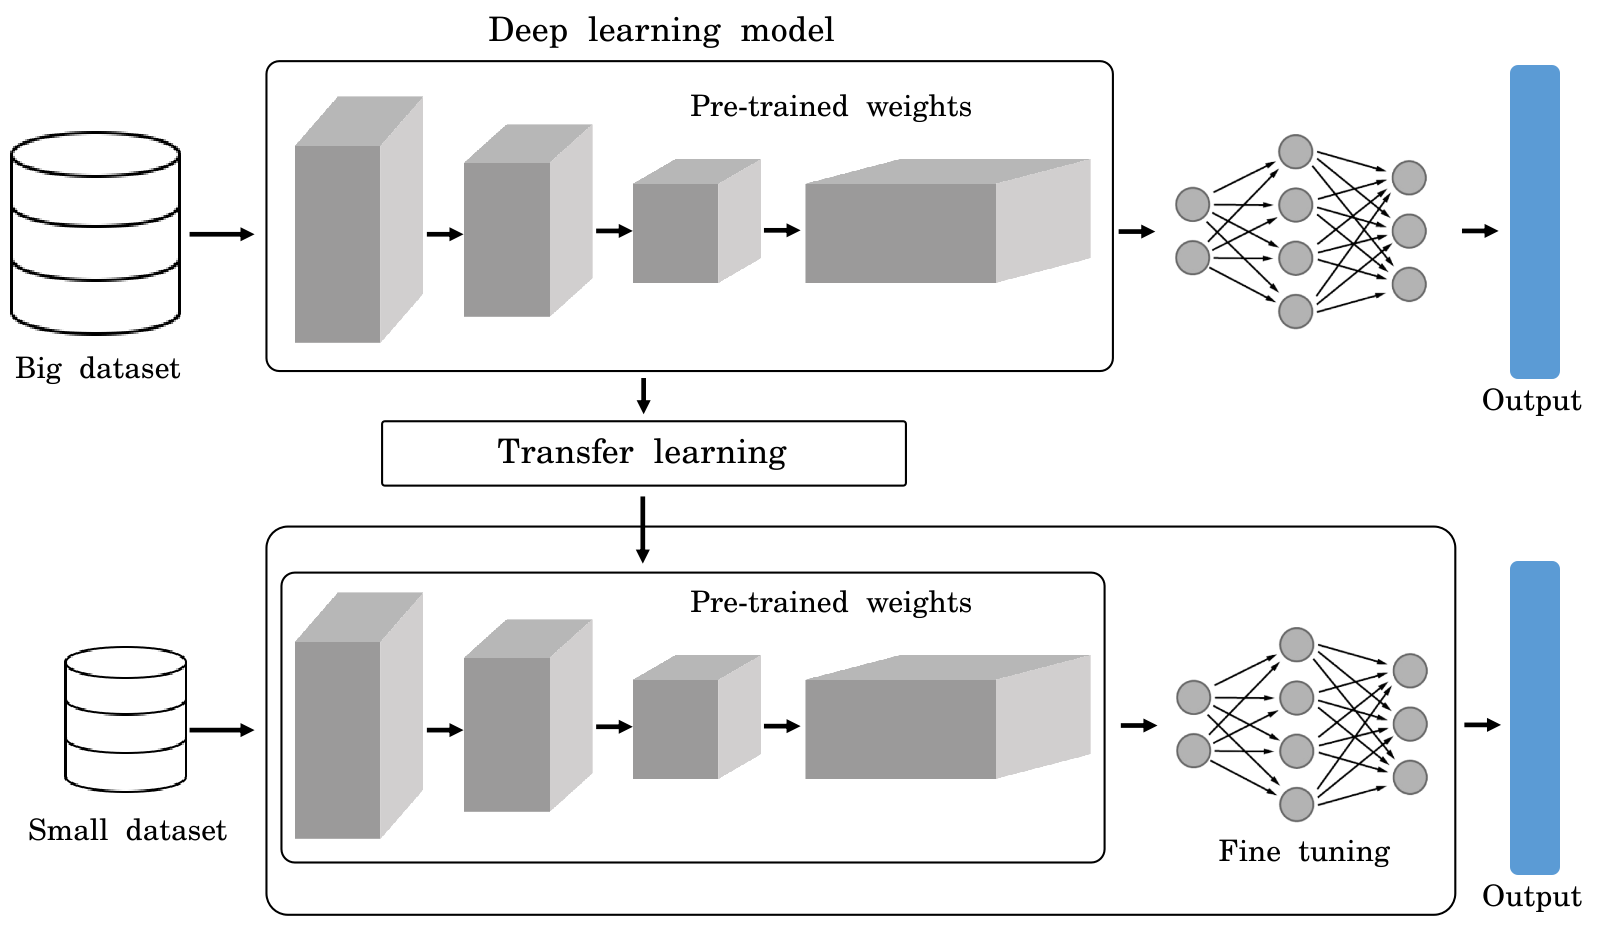
\includegraphics[width=\textwidth]{../img/proposal/fine_tuning}	
	\caption[Ejemplo de aplicación de \textit{Fine-tuning}]{Ejemplo de aplicación de \textit{Fine-tuning}. Primero, se entrena un modelo para una tarea $x$ con una gran base de datos, luego puede aprovecharse ese aprendizaje para otra tarea similar $y$ que no tenga una base de datos grande. Generalmente, en este proceso, se eliminan las ultimas capas y se agregan otras capas lineales, convoluciones o recurrentes. Fuente: Adaptado de  \cite{prince2023understanding}.}		
	\label{fig:fine-tuning}
\end{figure}


\begin{figure}[H]
	\centering
	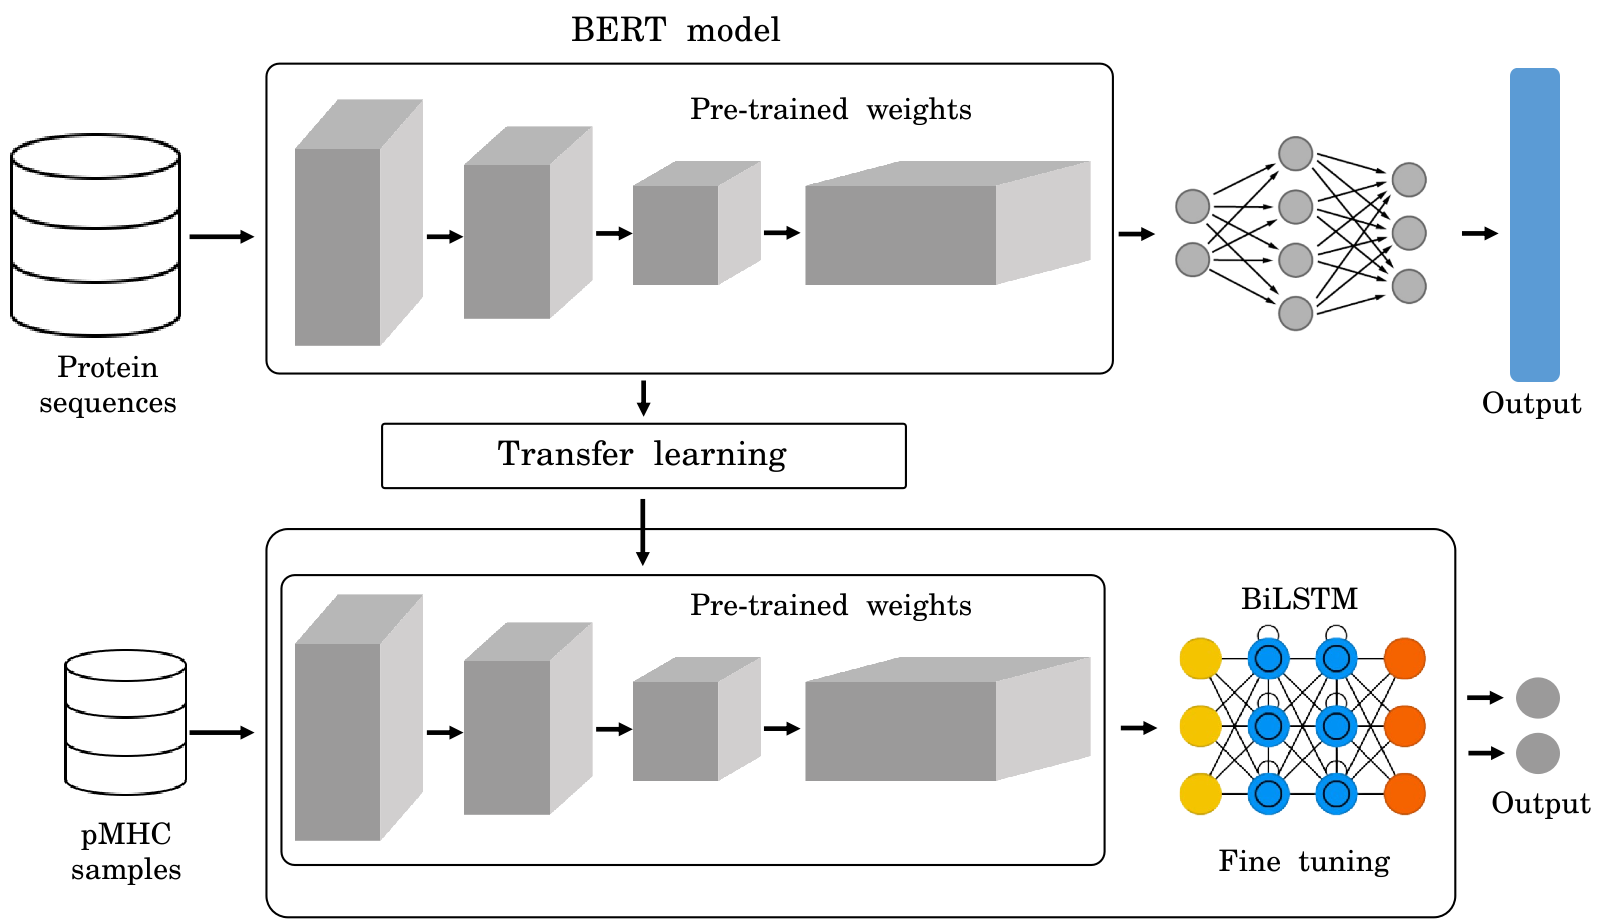
\includegraphics[width=\textwidth]{../img/proposal/fine_tuning_proposal}	
	\caption[Fine-tuning al modelo BERT]{\textit{Fine-tuning} propuesto. Se toma las primeras capas de un modelo BERT pre-entrenado con bases de datos de secuencias de proteínas. Luego, se agrega un bloque de capas BiLSTM al final y se entrena de nuevo con una base de datos pequeña de muestras pMHC. Fuente: Adaptado de  \cite{prince2023understanding}.}		
	\label{fig:fine-tuning_proposal}
\end{figure}
% agregar una figura especifica del finetuning




\begin{table}[t]%
	\centering
	\caption{Características del bloque BiLSTM utilizado en el \textit{fine-tuning}.}
	\label{tab:biLSTM}%
	\setlength{\tabcolsep}{0.5em} % for the horizontal padding
	{\renewcommand{\arraystretch}{1.5}% for the vertical padding
		\begin{tabular}{lp{9cm}p{1cm}p{1cm}}
			%\hline
			\textbf{Tipo}   & \textbf{Entada} & \textbf{Salida}& \textbf{Capas} \\ \hline
			
			BiLSTM & Salida del modelo BERT (Tabla \ref{tab:pretrained}, columna HS) & 768 & 2 \\ %\hline
			
			Dropout & 0.1\% & - & - \\
			Lineal & 1536 & 2 & 1 \\ %\hline
	\end{tabular}}
	
\end{table}





\section{\textit{Gradient Accumulation Steps}}\label{sec:gas}

Adicionalmente, los modelos de \textit{Transformer} grandes utilizan bastante memoria de la GPU. Por lo tanto, inspirados en trabajos similares sobre entrenamiento de modelos grandes de \textit{Transformers} para problemas de NLP \citep{anil2021large,zhang2023adam,huang2023measuring}, evaluamos los resultados de aplicar \textit{Gradient Accumulation Steps} durante el entrenamiento. El proceso se explica en la Figura \ref{fig:gas_example}, por ejemplo en un entrenamiento normal durante el proceso de actualización de parámetros en el algoritmo de aprendizaje, se considera un solo \textit{mini-batch} para obtener las gradientes y luego actualiza los parametros; mientras que en el enfoque utilizando \textit{Gradient Accumulation Steps}, se consideran varios \textit{mini-batchs}, se suman sus gradientes y luego estas gradientes acumuladas son utilizadas para actualizar los parámetros.



\begin{figure}[H]
	\centering
	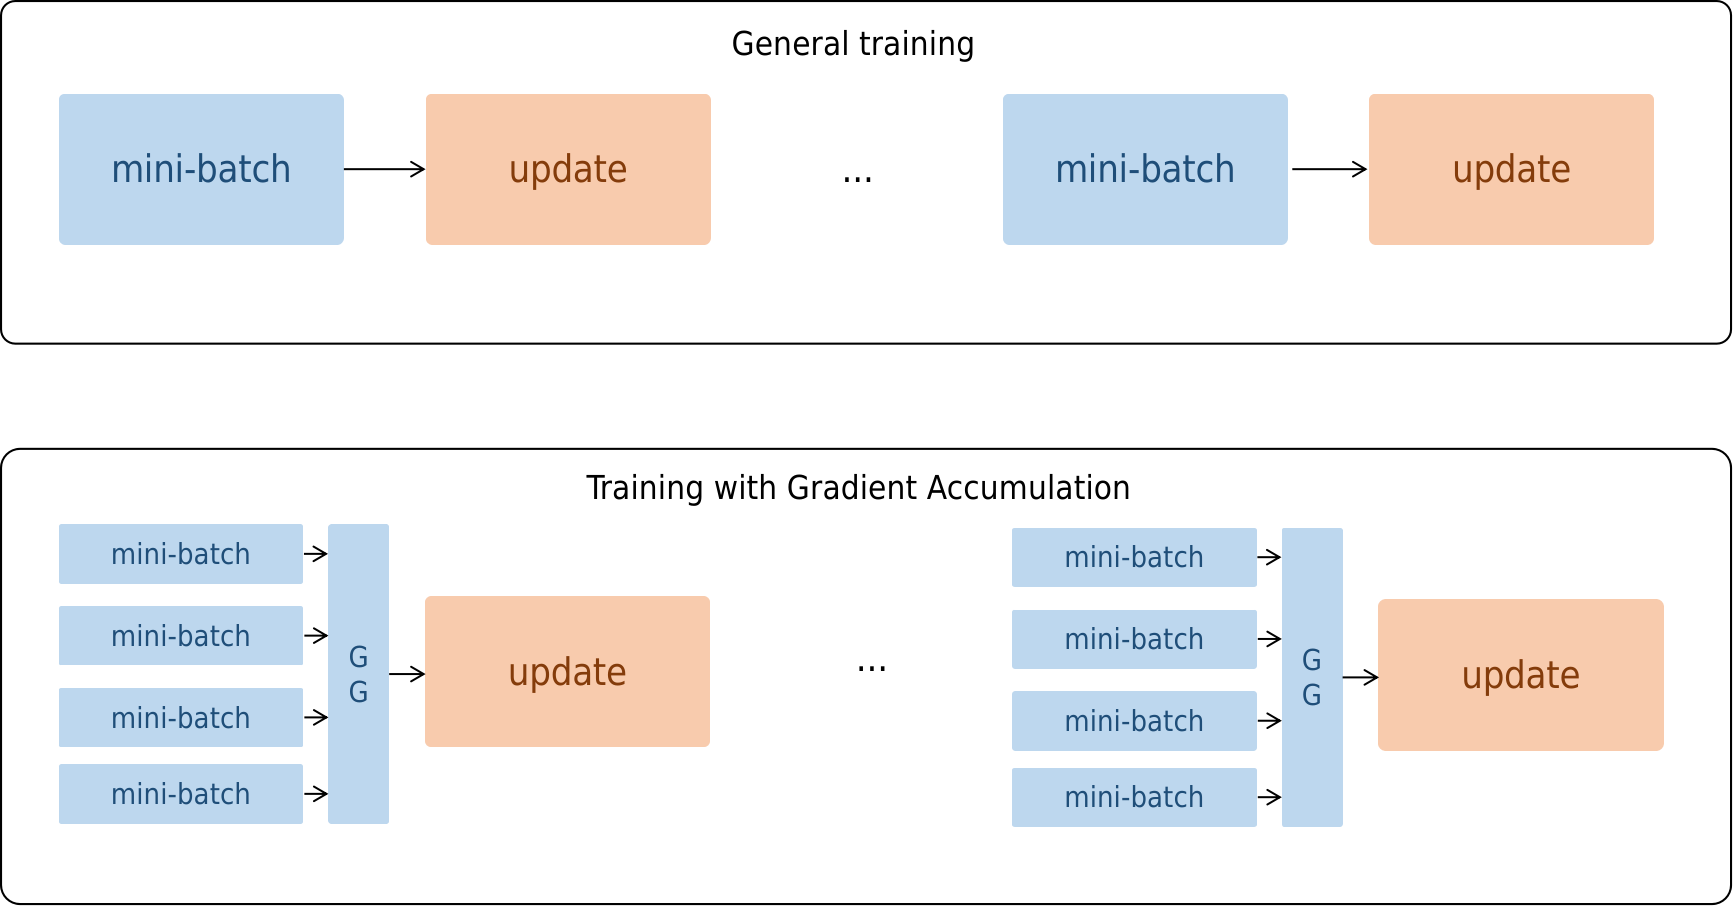
\includegraphics[width=\textwidth]{../img/proposal/gas_own}	
	\caption[Ejemplo de aplicación de \textit{Gradient Accumulation Steps}]{Ejemplo de aplicación de \textit{Gradient Accumulation Steps} durante el entranamiento de modelos de Deep Learning. En este caso, un entrenamiento general considera un solo \textit{mini-batch} para obtener las gradientes y luego actualiza los parámetros; mientras que en el enfoque utilizando \textit{Gradient Accumulation Steps}, se consideran varios \textit{mini-batchs}, se suman sus gradientes, luego estas gradientes acumuladas son utilizadas para actualizar los parámetros.  Fuente: Adaptado de  \cite{prince2023understanding}.}		
	\label{fig:gas_example}
\end{figure}

Generalmente, los parámetros de un modelo de \textit{machine learning} se actualizan según la ecuación \ref{equa:gas1}, donde $ \partial^i = \frac{\partial J(\theta)}{\partial \theta}   $ es la derivada partial de $\theta$ respecto a la función costo $J(\theta)$ en la iteración i. Entonces, el uso de \textit{Gradient Accumulation Steps} (GAS) propone acumular esas derivadas durante un número de iteraciones como se representa en la ecuación \ref{equa:gas2} (en este caso se acumuló las derivadas por tres iteraciones). Como resultado, al acumular las gradientes la actualización de parámetros se realiza cada cierto número de iteraciones reduciendo así el consumo de memoria. 

\begin{equation}\label{equa:gas1}
	\theta = \theta - \alpha \partial^{i}
\end{equation}

\begin{equation}\label{equa:gas2}
	\theta = \theta - \alpha (\partial^{i-1} + \partial^{i} + \partial^{i+1})
\end{equation}



En este proyecto, se planteo  comprobar los beneficios de utilizar GAS en el entrenamiento de los modelos. Se realizo una comparación de los modelos entrenados con GAS y sin GAS. Para los modelos TAPE, ESM2(t6), ESM2(t12) y ESM2(t30) se acumularón las gradientes por 64 iteraciones. Mientras que para los modelos mas grandes como ProtBert-BFD y ESM2(t33), se acumuló por 128 iteraciones. Se planteo esta diferencia porque los modelos mas grandes requerian un mayor consumo de memoria.


\section{Hiperparámetros}\label{sec:hyperparam}
Finalmente, utilizamos los siguientes hiperparámetros: tasa de aprendizaje de 5e-5, \textit{weight decay} de 0.0001, \textit{momentum} de 0.9, \textit{warn-up steps} de 1000 con \textit{linear decay}, optimizador ADAM ($\beta_1 = 0.9, \beta_2=0.999$). Estos valores fueron utilizados por BERTMHC \citep{cheng2021bertmhc} después de buscar los mejores parámetros utilizando \textit{grid search}. Adicionalmente, para los entrenamientos de mas de 30 \textit{epochs}, hemos aplicado  \textit{early stopping}. Esta técnica nos permite parar el entrenamiento si el desempeño no mejora despues de cierto número de \textit{epochs}, en este proyecto consideramos 5 \textit{epochs} como umbral para detener el entrenamiento.


\section{Conclusiones de la propuesta}

Como se detallo en este capítulo, la propuesta se basa en comparar metodologás de entrenamiento utilizando GAS y congelamiento de capas para realizar \textit{fine-tuning} a un modelo BERT pre-entrenado. El objetivo de \textit{fine-tuning}, es de adaptar el modelo BERT al problema de predicción del enlace pMHC.



